Quando esta dissertação teve início o projeto \acrshort{clav} já tinha cerca de 2 anos de 
desenvolvimento. Assim nesta secção será apresentado o estado da arte da 
\acrshort{clav} quando esta dissertação iniciou, aprofundando principalmente os pontos mais 
importantes sobre o tema desta dissertação. Além disso, serão apresentados os principais 
conceitos da \acrshort{clav} e iniciativas semelhantes a esta.

\section{Conceitos}

Para facilitar a compreensão e a leitura desta dissertação, explicam-se nesta secção os 
principais conceitos da \acrshort{clav}.

\subsection{Entidade}
Na \acrshort{clav} quando se faz referência a uma entidade esta é uma entidade pública. 
As entidades públicas intervêm nos processos de negócio podendo ter um de dois níveis de 
responsabilidade: uma entidade pode ser dona do processo ou participante no mesmo. 
Alguns exemplos de entidades públicas são hospitais públicos, escolas públicas, 
universidades públicas ou por exemplo, de forma mais específica, a Direção Geral de Viação, 
Instituto Nacional de Estatística, \acrlong{dglab}, entre outros.

\subsection{Tipologia}
Uma tipologia corresponde a um agrupamento de entidades públicas e surge no contexto deste projeto 
para facilitar algumas operações de associação e relacionamento que envolvem um grande número de entidades. 
Alguns exemplos são Agrupamentos de Centros de Saúde, Autarquias Locais, Forças Armadas, Embaixadas, entre outros.

\subsection{Legislação}
A legislação, no contexto da CLAV, corresponde ao conjunto de documentos legislativos que regulam ou condicionam as 
atividades desenvolvidas nos processos de negócio da administração pública e enquadram os prazos de conservação 
administrativa (\acrshort{pca}) e o destino final (\acrshort{df}) destes processos de negócio. 
O \acrshort{pca} é o período de tempo, registado em anos, durante o qual a informação deve ser mantida para 
responder a necessidades  de  negócio,  requisitos  organizacionais,  responsabilização  e obrigações 
legais~\cite{pca}. O \acrshort{df} é o destino final a dar à informação depois de cumprido o \acrshort{pca}. 
O \acrshort{df} pode ser de \emph{Conservação} (a documentação do processo tem que ser preservada em arquivo definitivo
ou histórico), de \emph{Conservação Parcial} (a documentação tem que ser preservada por amostragem, apenas uma
parte é preservada) ou de \emph{Eliminação} (a documentação é fisicamente eliminada sendo registada essa ação de 
eliminação).

\subsection{Processo de negócio}
Um \acrfull{pn} é uma sucessão ordenada de atividades interligadas, desempenhadas para atingir um resultado 
definido (produto ou serviço), no âmbito de uma função.~\cite{procNeg}

Na \acrshort{lc} o \acrshort{pn} é representado por uma classe de 3º nível que pode ser subdividida em classes de 
4º nível 
nos casos em que os vários documentos gerados ao logo das etapas do \acrlong{pn} possuam diferentes \acrshort{pca}'s 
e/ou diferentes \acrshort{df}'s.

Um exemplo de \acrshort{pn} é o processamento de matrículas ou inscrições no ensino ou em formação, ou seja, a 
realização ou renovação de matrícula em cursos ou inscrição em ações de formação. 
Este \acrshort{pn} inicia com o pedido de acesso ou ingresso e termina com a entrega de comprovativo de matrícula 
ou inscrição. Pelo meio possui etapas como a verificação de dados de identificação e validação da existência 
dos requisitos necessários para efeito de matrícula ou inscrição.

\subsection{Lista Consolidada}

A \acrfull{lc} é uma estrutura hierárquica de classes que representam as funções, subfunções e processos de 
negócio executados pela \acrfull{ap}, contemplando a sua descrição e avaliação.~\cite{lc}

Serve de referencial para a criação de instrumentos organizacionais ou pluriorganizacionais para a classificação e 
avaliação da informação pública (denominados \emph{Tabelas de Seleção}). 
Além disso é incremental pelo que ao longo do tempo o número de classes irá aumentar sendo este incremento da 
responsabilidade da \acrshort{dglab} que coordena e aprova a integração de novas classes.

A \acrshort{lc} permite:~\cite{lc}
\begin{itemize}
    \item O uso de uma linguagem comum na \acrshort{ap};
    \item Determinar a entidade responsável pela conservação permanente da informação;
    \item Partilhar e rentabilizar a informação;
    \item Racionalizar e agilizar processos;
    \item Controlar de forma mais eficaz os diferentes ciclos de vida informacional;
    \item Diminuir despesas correntes.
\end{itemize}

A \acrshort{lc} é o resultado de 3 projetos:
\begin{itemize}
    \item Projeto MEF - Macroestrutura Funcional: deste projeto resultaram os primeiros níveis (1º e 2º) da 
    \acrshort{lc} (funções e subfunções de administração) permitindo uma perspetiva global e integradora do 
    setor público;
    \item Projeto Harmonização de classes de 3.º nível em planos de classificação conformes à MEF: deste projeto 
    resultou a identificação e descrição dos processos de negócio da \acrshort{lc} (classes de nível 3);
    \item Projeto ASIA - Avaliação Suprainstitucional da Informação Arquivística: neste último projeto foi possível 
    estabelecer e associar  
    o \acrshort{pca} e \acrshort{df} a cada processo de negócio da \acrshort{lc}.
\end{itemize}

\subsection{Classificação}

A classificação arquivística é uma operação que visa a organização e representação da informação, tendo em vista a 
sua contextualização e garantir a sua autenticidade e integridade.~\cite{clavClass} 
Além disso é a base para a avaliação da informação, constituindo-se como condição para a eficácia e a eficiência 
administrativas.~\cite{clavClass} 
Esta classificação é suportada por um instrumento constituído por um esquema de classes pré-definidas e por um 
conjunto de regras ou instruções de aplicação (plano de classificação)~\cite{clavClass}.

\subsection{Avaliação}

A avaliação arquivística é uma operação que visa a atribuição de valor à informação arquivada, para efeitos de 
conservação ou de eliminação, fundamentada pelo \acrshort{pca} e pelo \acrshort{df}.~\cite{clavClass}

Tem por objetivo a implementação de boas práticas de gestão, a adequada conservação da informação que garante 
direitos e deveres e preserva a memória social e individual e a eliminação da informação desnecessária.~\cite{clavClass}

A avaliação é suportada por um instrumento denominado tabela de seleção (que é construído a partir da \acrshort{lc}).

\subsection{Tabela de Seleção}

Uma \acrfull{ts} é um instrumento de gestão onde se encontra:~\cite{tsDef}
\begin{itemize}
    \item a estrutura classificativa da informação, clarificando o seu âmbito e conteúdo (classificação)
    \item a definição do \acrlong{df} e do \acrlong{pca} e sua fundamentação (avaliação).
\end{itemize}

Uma \acrshort{ts} será sempre um subconjunto de classes da \acrshort{lc} para uma determinada 
entidade (\acrshort{ts} Organizacional) ou conjunto de entidades (\acrshort{ts} Pluriorganizacional) 
num determinado instante de tempo (a data da sua criação/aprovação). 
A aprovação das \acrshort{ts}'s é efetuada pela \acrshort{dglab}.

Enquanto a \acrshort{lc} está em constante mutação e atualização uma \acrshort{ts} fica congelada no tempo.
Poderão ser solicitadas alterações a uma \acrshort{ts} mas carecem sempre de uma aprovação por parte da DGLAB.


A \acrshort{clav} torna possível criar assistidamente as \acrshort{ts}'s evitando desde logo vários erros de 
utilizador e permitindo acelerar a criação destas.

A \acrshort{ts} pode integrar~\cite{tsDef}:
\begin{itemize}
    \item Portaria de Gestão de Documentos, quando aplicada à documentação ativa;
    \item Relatório  de  Avaliação  de  Documentação  Acumulada, quando aplicada às massas documentais acumuladas 
    não contempladas em Portaria de Gestão de Documentos.
\end{itemize}

Através da aplicação de uma \acrshort{ts} (classificação e avaliação) nos documentos produzidos 
(em suporte papel, eletrónico ou outro) de uma entidade é possível perceber que documentos devem ser conservados, 
e durante quanto tempo, ou eliminados. A eliminação de documentos sem necessidade de conservação permite 
disponibilizar meios e recursos para a conveniente gestão e conservação da documentação/informação produzida 
que precisa efetivamente de ser conservada de modo permanente.~\cite{ts}

\subsection{Donos e participantes de um \acrlong{pn}}

Os \acrshort{pn}'s podem ser executados por uma entidade ou várias entidades que podem ter diversos tipos de 
intervenção. A intervenção das entidades pode ser de dono (a entidade é responsável pela condução do \acrshort{pn}, 
pelo produto final e por garantir a conservação da informação) ou de participante (a entidade contribui para o 
desenvolvimento do \acrshort{pn} e do produto final).

\subsection{Autos de Eliminação}

Após serem selecionados os documentos a eliminar, aqueles cujo \acrshort{pca} já terminou e o \acrshort{df} é de 
eliminação, deve ser preenchido um \acrfull{ae}. O \acrshort{ae} serve para controlar a eliminação dos 
documentos das entidades e serve de prova de abate patrimonial. Além disso, deve ser transmitido à 
\acrshort{dglab} e constitui uma garantia de transparência da ação administrativa, bem como da capacidade do 
Estado no cumprimento da sua missão~\cite{pca}. 

Só após a \acrshort{dglab} confirmar que não existem 
inconformidades no \acrshort{ae} é que a entidade pode eliminar os documentos digitais e/ou físicos.

\section{O papel da \acrshort{clav}}

A \acrshort{clav} tem como objetivo servir de suporte para a classificação e a avaliação da informação pública 
ao facilitar a elaboração dos planos de classificação e tabelas de seleção bem como a consulta da \acrshort{lc}, 
das entidades, das tipologias e da legislação. Além disso, permite a edição da \acrshort{lc} e desmaterializar 
os procedimentos de controlo de eliminação de informação através da recolha e análise de autos de eliminação.

\section{Iniciativas Semelhantes à \acrshort{clav}}

Existem várias iniciativas semelhantes à \acrshort{clav} que se descrevem resumidamente nesta secção.

\subsection{Iniciativa Finlandesa}
Na Finlândia usam uma ferramenta de gestão de registos chamada 
AMS\footnote{abreviação da palavra finlandesa ``arkistonmuodostussuunnitelma''} que adiciona metadados aos 
registos com pouca intervenção humana. Estes metadados indicam o controlo de acesso e o tempo de retenção de cada 
registo. Esta ferramenta identifica os registos criados e recebidos pela organização e indica como devem ser 
manuseados. 

O \textit{core} desta ferramenta é um esquema de classificação funcional, o que possui algumas semelhanças com a 
\acrshort{lc}. Assim, quando um registo é adicionado a um \acrfull{erms} os valores \textit{default} 
dos metadados vêm do AMS. Em alguns casos é necessário alterar o valor \textit{default} manualmente visto que o 
sistema nem sempre consegue determinar as restrições de acesso de um registo.

Portanto um utilizador tem de operar tanto no esquema de classificação funcional como no \acrshort{erms}. 
Os utilizadores podem achar o esquema de classificação e o \acrshort{erms} difícil de entender e de 
usar~\cite{finInit} e como tal, há a necessidade por parte da iniciativa de tornar o processo de seleção mais 
fácil ou automatizá-lo. 

No artigo~\cite{finInit} é desenvolvida mais a fundo esta iniciativa dando possíveis soluções para o problema 
anteriormente descrito.

\subsection{Iniciativa da Universidade \textit{Victoria} de Toronto, Canadá}

A Universidade \textit{Victoria} criou um esquema de classificação com o intuito de classificar os registos da 
sua universidade. Para tal, usa dois princípios, a classificação funcional e a classificação multi nível. 
O primeiro organiza os registos pelo tipo de funções (finanças, administração, recursos humanos, etc) com os quais 
está relacionado. Quanto à classificação multi nível, os registos são organizados por 3 níveis de classificação. 
No primeiro nível é dividido pelas principais funções da universidade (classificação funcional). 
No segundo nível subdivide-se a função nas principais atividades (por exemplo a função de finanças inclui: 
auditoria, taxas, contabilidade, procuração, etc). Por fim, o terceiro nível divide cada atividade num tipo de 
registo com as suas diretrizes especificas de retenção e de disposição (destruição ou conservação). 
Por exemplo, a contabilidade das finanças inclui gestão de contas, contas a pagar, etc. 
O terceiro nível pode possuir mais divisões dependendo do número de registos.~\cite{uniInit} 

Este esquema encontra-se ainda em desenvolvimento e apresenta-se num estado inicial e apenas aplicável a alguns 
casos específicos.

Se compararmos com a \acrshort{lc} percebe-se que as duas são muitos semelhantes. 
Mas este esquema, que se aplica a uma entidade (a Universidade \textit{Victoria}), é ainda mais semelhante a 
uma \acrshort{ts} visto que as \acrshort{ts}'s aplicam-se a uma entidade ou conjunto de entidades.

\subsection{Comparação com a \acrshort{clav}}

As várias iniciativas aqui descritas encontram-se todas numa fase embrionária ou sem uma aplicação real sobre os 
documentos/registos. As várias razões para tal são o facto de possuírem demasiados processos de negócio/tipos de 
registo (o que torna o processo de classificação e de avaliação muito difícil ou impossível em termos práticos) 
ou porque ainda não chegaram a uma fase final de aplicação real.

Quanto à \acrshort{clav}, apesar de a \acrshort{lc} não se encontrar num estado final, encontra-se perto, e num 
estado passível de ser aplicado à vida real para várias entidades. Além disso, a \acrshort{clav} possui neste 
momento cerca de 1000 processos de negócio e com o tempo deve chegar no máximo a cerca de 2000 processos de negócio, 
um número gerível de processos de negócio.

Em Portugal, a \acrshort{lc} suportada pela \acrshort{clav} será em termos legislativos o instrumento oficial 
para a gestão da informação das entidades públicas. Haverá um período de transição que será também auxiliado pela 
plataforma \acrshort{clav} através da disponibilização dos \acrshort{rada}~\cite{rada}.

\section{Estrutura da plataforma CLAV}
A \acrshort{clav} está dividida em duas partes:
\begin{itemize}
    \item interface (\textit{front-end}) acessível em \url{http://clav.dglab.gov.pt};
    \item \acrshort{api} de dados (\textit{back-end} que inclui também duas bases de dados, \textit{GraphDB} e 
    \textit{MongoDB}) acessível em \url{http://clav-api.dglab.gov.pt}.
\end{itemize}

Através da figura~\ref{fig:clav_struct} é possível ver o possível fluxo tanto de um utilizador a aceder à 
interface como a de um utilizador a aceder diretamente à \acrshort{api} de dados. 

No primeiro caso, quando um utilizador acede o servidor da interface da \acrshort{clav} é descarregado para o 
lado do utilizador o ficheiro \acrshort{html} (\textit{index}) e os vários ficheiros \textit{JavaScript}, 
\acrshort{css} e \textit{assets} (como imagens, \acrshort{pdf}s, etc) quando necessários. 
O servidor da interface é nada mais que um servidor \textit{web} com recurso ao \textit{Nginx} que hospeda 
estes ficheiros, os quais representam a interface construída com o \textit{Vue} e o \textit{Vuetify}. 
Como tal o código apresenta-se todo do lado do utilizador sendo os pedidos à \acrshort{api} realizados do 
computador do utilizador para o servidor da \acrshort{api} de dados sem a intervenção do servidor da interface. 
Ou seja, o fluxo de cada um desses pedidos será igual ao fluxo no caso em que se acede diretamente à 
\acrshort{api} sem uso de qualquer interface como se pode observar na figura~\ref{fig:clav_struct}.

\begin{figure}[H]
    \centering
    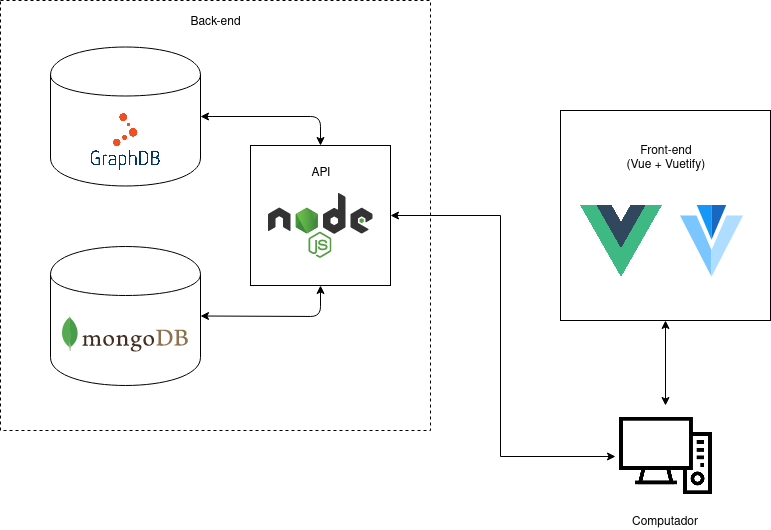
\includegraphics[width=0.7\textwidth]{img/clav_struct.png}
    \caption{Estrutura da \acrshort{clav} incluindo a interação de um utilizador com a mesma}\label{fig:clav_struct}
\end{figure}

Esta estrutura evoluiu depois para a estrutura presente na figura~\ref{fig:clav_struct2} em que continua a ser 
possível efetuar pedidos diretamente à \acrshort{api} de dados bem como obter a interface a partir do servidor 
da interface. Contudo passa a ser possível fazer os pedidos à \acrshort{api} de dados a partir do servidor da 
interface impedindo problemas de \acrshort{cors} ao efetuar pedidos a partir da interface localmente armazenada 
no cliente. Assim, o \textit{Nginx} reencaminha os pedidos que são para a \acrshort{api} de dados.

\begin{figure}[H]
    \centering
    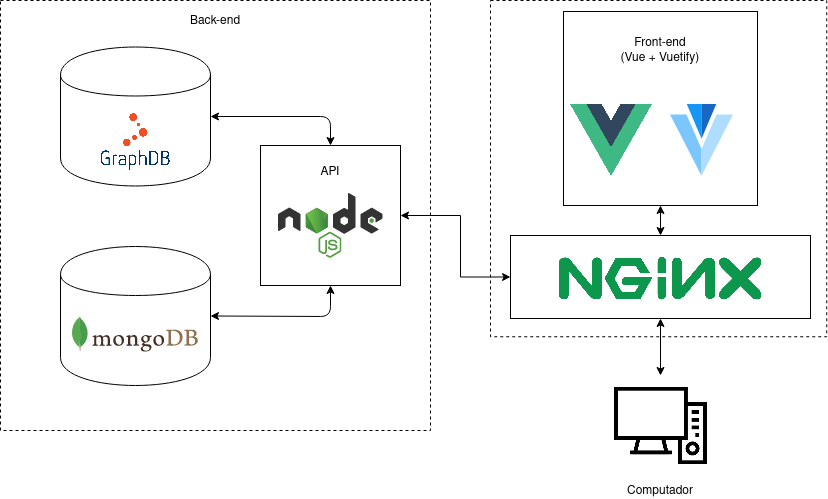
\includegraphics[width=0.7\textwidth]{img/clav_struct2.png}
    \caption{Estrutura evoluída da \acrshort{clav}}\label{fig:clav_struct2}
\end{figure}

Quanto à informação armazenada, no \textit{GraphDB} está presente a ontologia da \acrshort{clav} que contém a 
\acrshort{lc}, as entidades, as tipologias, a legislação entre outros dados. 

Por outro lado, no \textit{MongoDB} são guardados os utilizadores bem como outras informações importantes para a 
execução da \acrshort{api} de dados da \acrshort{clav}.

\section{Formas de autenticação}\label{sec:autenticacao}
A \acrshort{api} de dados e a interface estavam inicialmente juntas (aplicação monolítica) onde as rotas eram 
protegidas contudo, com a separação da aplicação em duas partes, ambas partes deixaram de estar protegidas. 
Devido à plataforma já ter estado protegida esta já possui duas formas de autenticação, através de chaves 
\acrshort{api} e através de utilizadores registados. Ou seja, tanto o registo de utilizadores e de chaves API já se 
encontra implementado bem como o \textit{login} de utilizadores.

As chaves \acrshort{api} existem por forma a dar acesso a certas rotas da \acrshort{api} a aplicações que 
interajam com a mesma (por exemplo sistemas de informação) sem a necessidade de interação humana.

Já os utilizadores possuem múltiplos níveis de acesso sendo que consoante o seu nível podem ou não aceder a uma 
rota da interface ou da \acrshort{api}. Os utilizadores podem autenticar-se através de \textit{email} e 
\textit{password} ou com recurso ao \acrfull{cc} através do Autenticação.gov, este último apenas disponível através da interface da \acrshort{clav}.

A hierarquia dos níveis de acesso, do nível que permite menor para o maior acesso, é a seguinte:
\begin{itemize}
    \item Nível 0: Chaves API,
    \item Nível 1: Representante Entidade,
    \item Nível 2: Utilizador Simples,
    \item Nível 3: Utilizador Arquivo Distrital,
    \item Nível 3.5: Utilizador Avançado,
    \item Nível 4: Utilizador Validador,
    \item Nível 5: Utilizador Decisor,
    \item Nível 6: Administrador de Perfil Funcional,
    \item Nível 7: Administrador de Perfil Tecnológico.
\end{itemize}

As chaves \acrshort{api} poderão aceder a algumas rotas com método \texttt{GET}.
Já os utilizadores poderão realizar todos os pedidos que as chaves \acrshort{api} podem realizar mas quanto 
maior o seu nível de acesso mais rotas poderão aceder.

A proteção da \acrshort{api} de dados terá de ter esta hierarquia em conta.

\subsection{Registo}

Como já referido, tanto o registo de chaves \acrshort{api} como de utilizadores já se encontra implementado.

Para o registo de uma chave \acrshort{api} é necessário providenciar um nome, um email e a entidade a que pertence. 
Após o registo da chave a informação desta chave \acrshort{api} é mantida numa base de dados \textit{MongoDB}.

Um utilizador pode se registar através de \texttt{email + password} ou através do Autenticação.gov. 
No primeiro caso, ao se registar necessita obviamente de indicar o seu email, a \textit{password}, o seu nome, 
a entidade a que pertence e o nível de acesso que pretende. 
Já no caso do Autenticação.gov para o registo do utilizador é necessário todos os campos anteriores exceto a 
\textit{password} (pode ser depois definida), sendo também necessário o campo \acrfull{nic} do utilizador. 
Caso o registo seja efetuado com recurso à interface do Autenticação.gov apenas será necessário indicar o email, 
a entidade a que pertence e o nível de acesso que pretende visto que os restantes campos são fornecidos pela 
Autenticação.gov quando o utilizador se autentica e autoriza a partilha dessa informação com a plataforma
\acrshort{clav}.
A \textit{password} é armazenada não na sua forma literal mas sim codificada numa \textit{hash} com a função 
criptográfica \texttt{bcrypt}. A utilização de funções de \textit{hash} criptográficas ao armazenar 
\textit{passwords} impede que as \textit{passwords} originais se saibam caso a base de dados seja comprometida. 
Para além disso, como o \texttt{bcrypt} combina um valor aleatório (\texttt{salt}) com a \textit{password} do 
utilizador, é impossível pré-computar a \textit{password} que deu origem ao \textit{hash} sem saber o 
\texttt{salt}\footnote{Para mais informação veja \textit{rainbow table attack}}.

Durante esta tese com a proteção da \acrshort{api} de dados ficará apenas possível o registo de utilizadores 
através de utilizadores que já estejam registados e possuam um nível de acesso suficiente para registar 
utilizadores. Estes utilizadores registados e autorizados pertencem à entidade \acrshort{dglab}. 
Portanto, utilizadores representantes de outras entidades que queiram registar-se na plataforma terão de:~\cite{clavwebpage}
\begin{itemize}
    \item Preencher o formulário disponibilizado para o efeito, para cada representante designado pela entidade;
    \item O formulário deverá ser assinado por um dirigente superior da Entidade e autenticado com assinatura digital, se o envio for feito por via eletrónica (NB\@: não serão aceites assinaturas do formulário por dirigentes intermédios). Esta autorização autenticada pelo dirigente superior é o equivalente a uma delegação de competências, uma vez que o representante da entidade passa a ter capacidade para, em nome da entidade, submeter autos de eliminação, propostas de tabelas de seleção e novas classes para a Lista Consolidada;
    \item O formulário deverá ser remetido à \acrshort{dglab} por via postal ou eletrónica, respetivamente, para:
    \begin{itemize}
        \item \acrshort{dglab}, Edifício da Torre do Tombo, Alameda da Universidade, 1649--010 Lisboa (formulário assinado manualmente) ou
        \item clav@dglab.gov.pt (formulário com assinatura digital).
    \end{itemize}
    \item Após receção do formulário, a \acrshort{dglab} efetuará o(s) respetivo(s) registo(s) até 48 horas úteis;
    \item Findo esse prazo, o utilizador poderá aceder à plataforma, selecionando a opção ``Autenticação'';
    \item A autenticação, no primeiro acesso, deve ser efetuada com o \acrlong{cc}.
\end{itemize}

\subsection{\textit{Login}}

O \textit{login} apenas está presente para o caso dos utilizadores visto que, assim que uma chave \acrshort{api} 
é registada, é enviado por email um \acrshort{jwt} com a duração de 30 dias a ser usado nos pedidos a realizar 
à \acrshort{api} de dados. O utilizador poderá ao fim dos 30 dias renovar a sua chave \acrshort{api}, onde é 
gerado um novo \acrshort{jwt}.

Portanto do lado dos utilizadores é possível como já referido realizar o \textit{login} de duas formas através de 
uma estratégia local ou através do Autenticação.gov.

A estratégia local (\texttt{email + password}) é conseguida através do uso do \textit{middleware} \textit{Passport}.
O \textit{Passport} é um \textit{middleware} de autenticação para \textit{Node.js} que tem como objetivo autenticar 
pedidos.~\cite{passport} Tem como única preocupação a autenticação delegando qualquer outra funcionalidade para a 
aplicação que a usa. Este \textit{middleware} possui muitas estratégias de autenticação entre as quais a 
local (\texttt{email/username + password}), \acrshort{jwt}, \textit{OAuth}\footnote{Protocolo \textit{open-source} 
com o objetivo de permitir a autenticação simples, segura e padrão entre aplicações móveis, \textit{web} e 
\textit{desktop}}, \textit{Facebook} ou \textit{Twitter}. Cada estratégia está num módulo independente. 
Assim as aplicações que usam o \textit{Passport} não terão um peso adicional devido a estratégias que nem sequer usam.

No caso do \textit{login} através do Autenticação.gov, o utilizador tem de se autenticar na interface do 
Autenticação.gov (a partir do botão disponível na área de autenticação da interface do \acrshort{clav}). 
O fluxo do \textit{login} antes da limitação do registo de utilizadores apenas por pessoal autorizado pode ser observado na figura~\ref{fig:authgov}:

\begin{figure}[H]
    \centering
    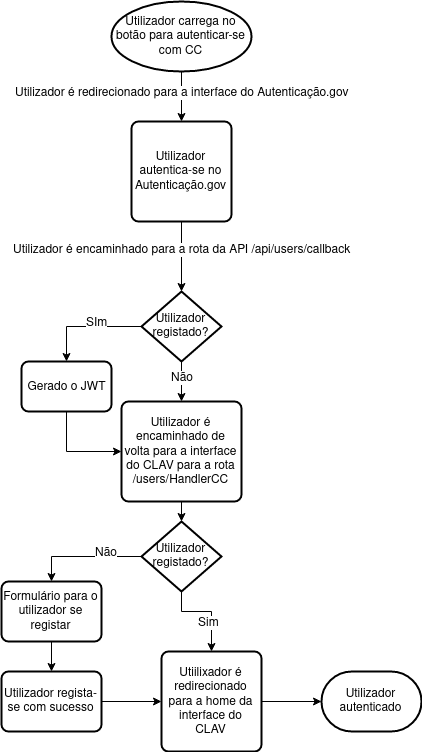
\includegraphics[width=0.5\textwidth]{img/authgov.png}
    \caption{Fluxo do \textit{login} de um utilizador através do Autenticação.gov antes da limitação do registo de utilizadores apenas por pessoal autorizado}\label{fig:authgov}
\end{figure}

Após a limitação do registo de utilizadores apenas por pessoal autorizado continuará a ser possível o utilizador 
autenticar-se pelo Autenticação.gov mas deixará de ser possível o utilizador registar-se aparecendo, em vez de 
um formulário de registo, um aviso de que o utilizador não se encontra registado.

No \textit{login} do utilizador é gerado um \acrshort{jwt} com a duração de 8 horas que deve ser usado nos pedidos 
a realizar à \acrshort{api} de dados. No fim das 8 horas o utilizador necessita de se autenticar de novo.

\section{Resumo}

Neste capítulo foi brevemente abordada a \acrshort{clav}, explicando os principais conceitos desta que irão ajudar 
a compreender algumas das secções seguintes desta dissertação.

Além disso, foi efetuada uma breve descrição de iniciativas semelhantes com a \acrshort{clav} comparando-as a esta.

Por fim, foi descrito a estrutura e as formas de autenticação (registo e \textit{login}) da \acrshort{clav} no 
momento que esta dissertação iniciou com o objetivo de o leitor perceber que trabalho tem de ser efetuado e a 
razão de algumas decisões e implementações efetuadas nesta dissertação.
